\begin{subfigure}[b]{.3\textwidth}
	\renewcommand\thesubfigure{\alph{subfigure}1}
	\centering
	\resizebox{\textwidth}{!}{
	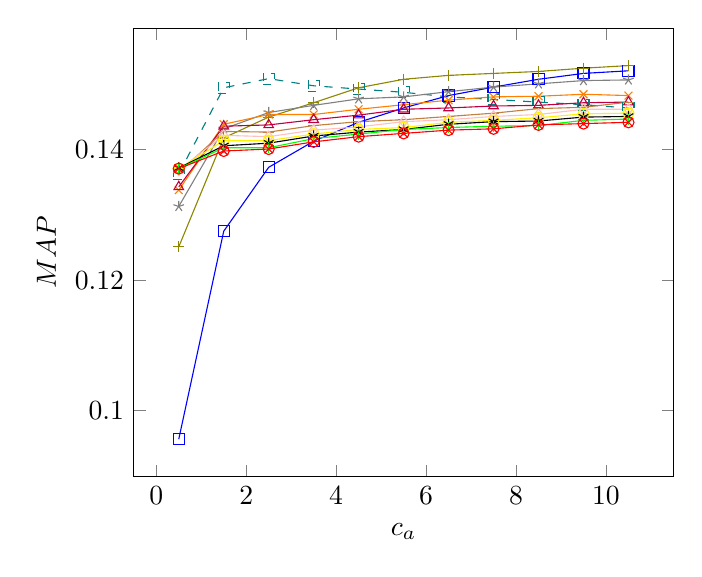
\begin{tikzpicture}
		\begin{axis}[
		xlabel=$c_a$,
		ylabel=$MAP$,
		% y label style={rotate=-90}
	]
%%%%%%%%%%%%%%%%%%%%
%%% x=cv y=ca, from 5 to 50, with step of 5
%%%%%%%%%%%%%%%%%%%%
%%\addplot[mark=square, style=solid, color=blue] coordinates

%\addplot[mark=+, style=solid, color=olive] coordinates
%{ (0, 0.1492) (5, 0.1451) (10, 0.1425) (15, 0.1411) (20, 0.1397) (25, 0.1381) (30, 0.1373) (35, 0.137) (40, 0.1365) (45, 0.136) (50, 0.1356) };

%\addplot[mark=star, style=solid, color=gray] coordinates
%{ (0, 0.1468) (5, 0.1469) (10, 0.1444) (15, 0.1421) (20, 0.1408) (25, 0.1397) (30, 0.1387) (35, 0.1381) (40, 0.1377) (45, 0.1372) (50, 0.1369) };

%\addplot[mark=x, style=solid, color=orange] coordinates
%{ (0, 0.1452) (5, 0.1476) (10, 0.1442) (15, 0.1419) (20, 0.1407) (25, 0.1397) (30, 0.1388) (35, 0.1382) (40, 0.1377) (45, 0.1373) (50, 0.1369) };

%\addplot[mark=triangle, style=solid, color=purple] coordinates
%{ (0, 0.1443) (5, 0.1475) (10, 0.1435) (15, 0.1415) (20, 0.1403) (25, 0.1393) (30, 0.1384) (35, 0.1379) (40, 0.1375) (45, 0.1371) (50, 0.1369) };

%\addplot[mark=-, style=solid, color=brown] coordinates
%{ (0, 0.1431) (5, 0.1472) (10, 0.1435) (15, 0.1413) (20, 0.1399) (25, 0.139) (30, 0.1384) (35, 0.1378) (40, 0.1374) (45, 0.1371) (50, 0.1367) };

%\addplot[mark=diamond, style=solid, color=pink] coordinates
%{ (0, 0.1422) (5, 0.1472) (10, 0.1432) (15, 0.1412) (20, 0.1401) (25, 0.1393) (30, 0.1385) (35, 0.1379) (40, 0.1376) (45, 0.1372) (50, 0.137) };

%\addplot[mark=oplus, style=solid, color=yellow] coordinates
%{ (0, 0.1418) (5, 0.1473) (10, 0.1431) (15, 0.1411) (20, 0.1401) (25, 0.1392) (30, 0.1387) (35, 0.1383) (40, 0.1378) (45, 0.1374) (50, 0.137) };

%\addplot[mark=asterisk, style=solid, color=black] coordinates
%{ (0, 0.141) (5, 0.147) (10, 0.1431) (15, 0.1411) (20, 0.1402) (25, 0.1392) (30, 0.1389) (35, 0.1383) (40, 0.1378) (45, 0.1373) (50, 0.137) };

%\addplot[mark=|, style=solid, color=green] coordinates
%{ (0, 0.1406) (5, 0.1468) (10, 0.143) (15, 0.1413) (20, 0.1403) (25, 0.1394) (30, 0.1387) (35, 0.1382) (40, 0.1377) (45, 0.1372) (50, 0.1369) };

%\addplot[mark=otimes, style=solid, color=red] coordinates
%{ (0, 0.1403) (5, 0.1466) (10, 0.1431) (15, 0.1412) (20, 0.1402) (25, 0.1394) (30, 0.1386) (35, 0.1383) (40, 0.1379) (45, 0.1373) (50, 0.1368) };

%%%%%%%%%%%%%%%%%%%%
%%% x=ca y=cv, from 0.5 to 10.5, with step of 1
%%%%%%%%%%%%%%%%%%%%
\addplot[mark=square, style=dashed, color=teal] coordinates
{ (0.5, 0.1363) (1.5, 0.1495) (2.5, 0.1509) (3.5, 0.1498) (4.5, 0.1493) (5.5, 0.1488) (6.5, 0.1481) (7.5, 0.1477) (8.5, 0.1473) (9.5, 0.1469) (10.5, 0.1464) };

\addplot[mark=square, style=solid, color=blue] coordinates
{ (0.5, 0.0956) (1.5, 0.1275) (2.5, 0.1373) (3.5, 0.1413) (4.5, 0.1442) (5.5, 0.1464) (6.5, 0.1483) (7.5, 0.1496) (8.5, 0.1508) (9.5, 0.1517) (10.5, 0.1521) };

\addplot[mark=+, style=solid, color=olive] coordinates
{ (0.5, 0.1251) (1.5, 0.1418) (2.5, 0.145) (3.5, 0.1472) (4.5, 0.1495) (5.5, 0.1508) (6.5, 0.1514) (7.5, 0.1517) (8.5, 0.152) (9.5, 0.1525) (10.5, 0.1529) };

\addplot[mark=star, style=solid, color=gray] coordinates
{ (0.5, 0.1313) (1.5, 0.1432) (2.5, 0.1457) (3.5, 0.1468) (4.5, 0.1478) (5.5, 0.1481) (6.5, 0.1489) (7.5, 0.1496) (8.5, 0.1501) (9.5, 0.1506) (10.5, 0.1507) };

\addplot[mark=x, style=solid, color=orange] coordinates
{ (0.5, 0.1338) (1.5, 0.1439) (2.5, 0.1454) (3.5, 0.1454) (4.5, 0.1462) (5.5, 0.1469) (6.5, 0.1476) (7.5, 0.1481) (8.5, 0.1482) (9.5, 0.1485) (10.5, 0.1483) };

\addplot[mark=triangle, style=solid, color=purple] coordinates
{ (0.5, 0.1343) (1.5, 0.1436) (2.5, 0.1438) (3.5, 0.1446) (4.5, 0.1453) (5.5, 0.1462) (6.5, 0.1464) (7.5, 0.1467) (8.5, 0.1468) (9.5, 0.1472) (10.5, 0.1473) };

\addplot[mark=-, style=solid, color=brown] coordinates
{ (0.5, 0.1365) (1.5, 0.1428) (2.5, 0.1427) (3.5, 0.1437) (4.5, 0.1443) (5.5, 0.1446) (6.5, 0.1451) (7.5, 0.1456) (8.5, 0.1463) (9.5, 0.1465) (10.5, 0.1473) };

\addplot[mark=diamond, style=solid, color=pink] coordinates
{ (0.5, 0.1369) (1.5, 0.1422) (2.5, 0.142) (3.5, 0.143) (4.5, 0.1435) (5.5, 0.1443) (6.5, 0.1446) (7.5, 0.1451) (8.5, 0.1454) (9.5, 0.1462) (10.5, 0.1462) };

\addplot[mark=oplus, style=solid, color=yellow] coordinates
{ (0.5, 0.1371) (1.5, 0.1414) (2.5, 0.1414) (3.5, 0.1424) (4.5, 0.1431) (5.5, 0.1434) (6.5, 0.1442) (7.5, 0.1445) (8.5, 0.1449) (9.5, 0.1455) (10.5, 0.1456) };

\addplot[mark=asterisk, style=solid, color=black] coordinates
{ (0.5, 0.1372) (1.5, 0.1406) (2.5, 0.141) (3.5, 0.1421) (4.5, 0.1427) (5.5, 0.1431) (6.5, 0.1439) (7.5, 0.1443) (8.5, 0.1444) (9.5, 0.145) (10.5, 0.1451) };

\addplot[mark=|, style=solid, color=green] coordinates
{ (0.5, 0.1371) (1.5, 0.1403) (2.5, 0.1403) (3.5, 0.1417) (4.5, 0.1424) (5.5, 0.1431) (6.5, 0.1434) (7.5, 0.1436) (8.5, 0.1437) (9.5, 0.1445) (10.5, 0.1447) };

\addplot[mark=otimes, style=solid, color=red] coordinates
{ (0.5, 0.1371) (1.5, 0.1398) (2.5, 0.1401) (3.5, 0.1412) (4.5, 0.142) (5.5, 0.1425) (6.5, 0.143) (7.5, 0.1432) (8.5, 0.1438) (9.5, 0.144) (10.5, 0.1442) };

\end{axis}
\end{tikzpicture}}

	\caption{INEX09}
\end{subfigure}
\quad%
\begin{subfigure}[b]{.3\textwidth}
	\addtocounter{subfigure}{-1}
	\renewcommand\thesubfigure{\alph{subfigure}2}
	\centering
	\resizebox{\textwidth}{!}{
	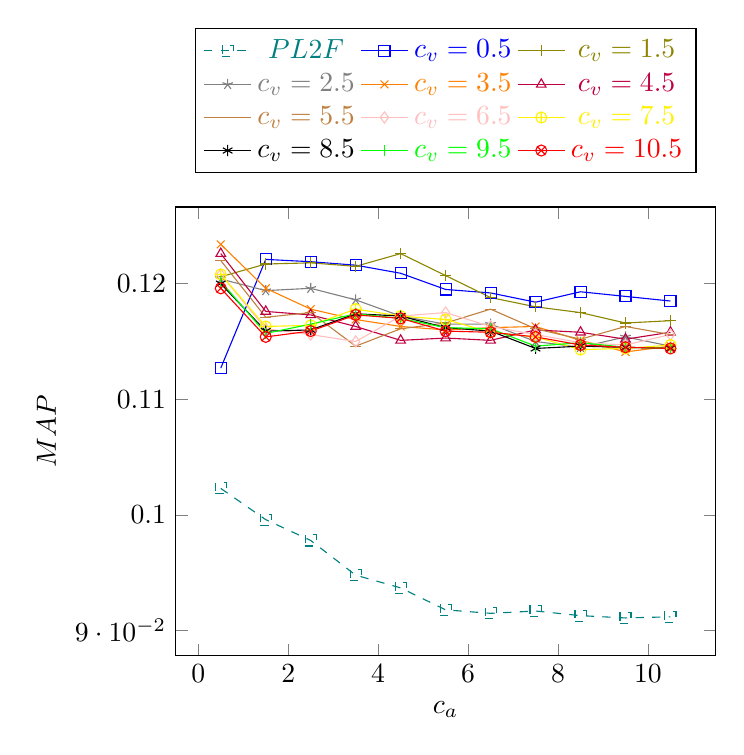
\begin{tikzpicture}
	\begin{axis}[
	  legend entries={
	    [teal]$PL2F$,
		[blue]$c_v = 0.5$,
	 	[olive]$c_v = 1.5$,
	  	[gray]$c_v = 2.5$,
	  	[orange]$c_v = 3.5$,
		[purple]$c_v = 4.5$,
	 	[brown]$c_v = 5.5$,
	  	[pink]$c_v = 6.5$,
	  	[yellow]$c_v = 7.5$,
		[black]$c_v = 8.5$,
	 	[green]$c_v = 9.5$,
	 	[red]$c_v = 10.5$
	  },
	  legend columns=3,
	legend style={at={(0.5,1.4)},anchor=north},
	 xlabel=$c_a$,
	ylabel=$MAP$,
	% y label style={rotate=-90},
	]

%%%%%%%%%%%%%%%%%%%%
%%% x=cv y=ca, from 5 to 50, with step of 5
%%%%%%%%%%%%%%%%%%%%
%\addplot[mark=square, style=solid, color=blue] coordinates
%{ (5, ) (10, ) (15, ) (20, ) (25, ) (30, ) (35, ) (40, ) (45, ) (50, )  };

%\addplot[mark=+, style=solid, color=olive] coordinates
%{ (0, 0.0928) (5, 0.1153) (10, 0.1174) (15, 0.116) (20, 0.1167) (25, 0.115) (30, 0.1136) (35, 0.1137) (40, 0.1139) (45, 0.1132) (50, 0.1136)  };

%\addplot[mark=star, style=solid, color=gray] coordinates
%{ (0, 0.0913) (5, 0.1158) (10, 0.1144) (15, 0.113) (20, 0.1136) (25, 0.114) (30, 0.1126) (35, 0.1127) (40, 0.112) (45, 0.1114) (50, 0.1106)  };

%\addplot[mark=x, style=solid, color=orange] coordinates
%{ (0, 0.0886) (5, 0.115) (10, 0.114) (15, 0.1127) (20, 0.1123) (25, 0.1123) (30, 0.1122) (35, 0.1121) (40, 0.1113) (45, 0.1105) (50, 0.1104)  };

%\addplot[mark=triangle, style=solid, color=purple] coordinates
%{ (0, 0.0879) (5, 0.114) (10, 0.1132) (15, 0.112) (20, 0.1124) (25, 0.1119) (30, 0.111) (35, 0.1111) (40, 0.1097) (45, 0.1097) (50, 0.1098)  };

%\addplot[mark=-, style=solid, color=brown] coordinates
%{ (0, 0.0868) (5, 0.1137) (10, 0.1137) (15, 0.1125) (20, 0.1111) (25, 0.1105) (30, 0.1101) (35, 0.11) (40, 0.1099) (45, 0.109) (50, 0.1091)  };

%\addplot[mark=diamond, style=solid, color=pink] coordinates
%{ (0, 0.0864) (5, 0.1131) (10, 0.1126) (15, 0.111) (20, 0.1104) (25, 0.1092) (30, 0.1092) (35, 0.1093) (40, 0.109) (45, 0.1081) (50, 0.1082)  };

%\addplot[mark=oplus, style=solid, color=yellow] coordinates
%{ (0, 0.0856) (5, 0.1129) (10, 0.1109) (15, 0.1105) (20, 0.1097) (25, 0.1084) (30, 0.1082) (35, 0.1076) (40, 0.1081) (45, 0.1079) (50, 0.107)  };

%\addplot[mark=asterisk, style=solid, color=black] coordinates
%{ (0, 0.0845) (5, 0.1124) (10, 0.1115) (15, 0.1102) (20, 0.1095) (25, 0.1083) (30, 0.1079) (35, 0.1078) (40, 0.1075) (45, 0.1073) (50, 0.1066)  };

%\addplot[mark=|, style=solid, color=green] coordinates
%{ (0, 0.0833) (5, 0.1121) (10, 0.1113) (15, 0.1099) (20, 0.1095) (25, 0.1087) (30, 0.1081) (35, 0.1081) (40, 0.1077) (45, 0.1068) (50, 0.1059)  };

%\addplot[mark=otimes, style=solid, color=red] coordinates
%{ (0, 0.0824) (5, 0.1116) (10, 0.1109) (15, 0.1099) (20, 0.1095) (25, 0.1086) (30, 0.1077) (35, 0.1077) (40, 0.1076) (45, 0.107) (50, 0.1068)  };

%%%%%%%%%%%%%%%%%%%%
%%% x=ca y=cv, from 0.5 to 10.5, with step of 1
%%%%%%%%%%%%%%%%%%%%
\addplot[mark=square, style=dashed, color=teal] coordinates
{ (0.5, 0.1023) (1.5, 0.0996) (2.5, 0.0978) (3.5, 0.0948) (4.5, 0.0937) (5.5, 0.0918) (6.5, 0.0915) (7.5, 0.0917) (8.5, 0.0913) (9.5, 0.0911) (10.5, 0.0912) };

\addplot[mark=square, style=solid, color=blue] coordinates
{ (0.5, 0.1127) (1.5, 0.1221) (2.5, 0.1219) (3.5, 0.1216) (4.5, 0.1209) (5.5, 0.1195) (6.5, 0.1192) (7.5, 0.1184) (8.5, 0.1193) (9.5, 0.1189) (10.5, 0.1185) };

\addplot[mark=+, style=solid, color=olive] coordinates
{ (0.5, 0.1206) (1.5, 0.1217) (2.5, 0.1218) (3.5, 0.1215) (4.5, 0.1226) (5.5, 0.1207) (6.5, 0.1188) (7.5, 0.118) (8.5, 0.1175) (9.5, 0.1166) (10.5, 0.1168) };

\addplot[mark=star, style=solid, color=gray] coordinates
{ (0.5, 0.1204) (1.5, 0.1194) (2.5, 0.1196) (3.5, 0.1186) (4.5, 0.1172) (5.5, 0.1165) (6.5, 0.1165) (7.5, 0.115) (8.5, 0.1145) (9.5, 0.1154) (10.5, 0.1146) };

\addplot[mark=x, style=solid, color=orange] coordinates
{ (0.5, 0.1234) (1.5, 0.1196) (2.5, 0.1178) (3.5, 0.1169) (4.5, 0.1163) (5.5, 0.116) (6.5, 0.1162) (7.5, 0.1163) (8.5, 0.1151) (9.5, 0.1141) (10.5, 0.1146) };

\addplot[mark=triangle, style=solid, color=purple] coordinates
{ (0.5, 0.1226) (1.5, 0.1176) (2.5, 0.1173) (3.5, 0.1163) (4.5, 0.1151) (5.5, 0.1153) (6.5, 0.1151) (7.5, 0.116) (8.5, 0.1158) (9.5, 0.1152) (10.5, 0.1158) };

\addplot[mark=-, style=solid, color=brown] coordinates
{ (0.5, 0.122) (1.5, 0.1171) (2.5, 0.1175) (3.5, 0.1146) (4.5, 0.1161) (5.5, 0.1166) (6.5, 0.1178) (7.5, 0.1161) (8.5, 0.1152) (9.5, 0.1163) (10.5, 0.1156) };

\addplot[mark=diamond, style=solid, color=pink] coordinates
{ (0.5, 0.1208) (1.5, 0.1161) (2.5, 0.1156) (3.5, 0.115) (4.5, 0.1172) (5.5, 0.1175) (6.5, 0.1163) (7.5, 0.1156) (8.5, 0.1149) (9.5, 0.1147) (10.5, 0.1156) };

\addplot[mark=oplus, style=solid, color=yellow] coordinates
{ (0.5, 0.1208) (1.5, 0.1163) (2.5, 0.1164) (3.5, 0.1178) (4.5, 0.1172) (5.5, 0.1169) (6.5, 0.1158) (7.5, 0.1154) (8.5, 0.1143) (9.5, 0.1144) (10.5, 0.1147) };

\addplot[mark=asterisk, style=solid, color=black] coordinates
{ (0.5, 0.12) (1.5, 0.1159) (2.5, 0.116) (3.5, 0.1174) (4.5, 0.1172) (5.5, 0.1162) (6.5, 0.1159) (7.5, 0.1144) (8.5, 0.1146) (9.5, 0.1145) (10.5, 0.1144) };

\addplot[mark=|, style=solid, color=green] coordinates
{ (0.5, 0.1202) (1.5, 0.1157) (2.5, 0.1165) (3.5, 0.1174) (4.5, 0.117) (5.5, 0.1162) (6.5, 0.1161) (7.5, 0.1146) (8.5, 0.1149) (9.5, 0.1145) (10.5, 0.1144) };

\addplot[mark=otimes, style=solid, color=red] coordinates
{ (0.5, 0.1196) (1.5, 0.1154) (2.5, 0.1159) (3.5, 0.1173) (4.5, 0.117) (5.5, 0.1159) (6.5, 0.1158) (7.5, 0.1154) (8.5, 0.1147) (9.5, 0.1145) (10.5, 0.1144) };

\end{axis}
\end{tikzpicture}}

	\caption{SS10}
\end{subfigure}
\quad%
\begin{subfigure}[b]{.3\textwidth}
	\addtocounter{subfigure}{-1}
	\renewcommand\thesubfigure{\alph{subfigure}3}
	\centering
	\resizebox{\textwidth}{!}{
	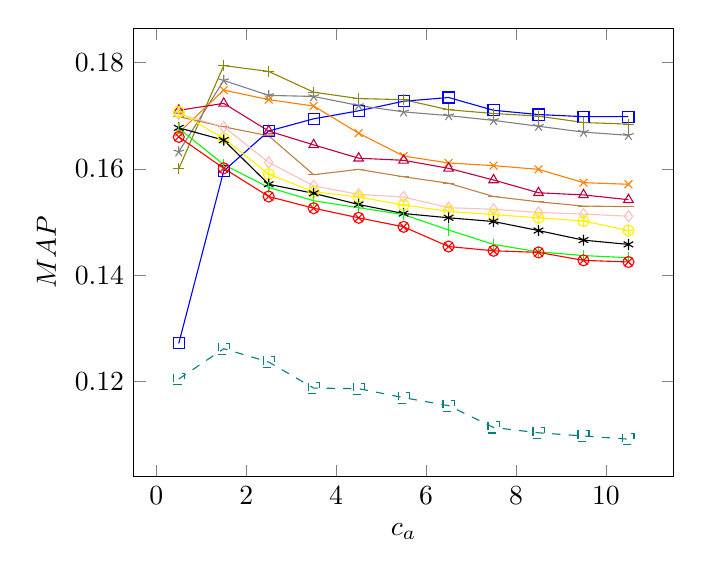
\begin{tikzpicture}
	\begin{axis}[
	 xlabel=$c_a$,
	ylabel=$MAP$,
	% y label style={rotate=-90},
	]

%%%%%%%%%%%%%%%%%%%%
%%% x=cv y=ca, from 5 to 50, with step of 5
%%%%%%%%%%%%%%%%%%%%
%%\addplot[mark=square, style=solid, color=blue] coordinates
%%{ ( , ) ( , ) ( , ) ( , ) ( , ) ( , ) ( , ) ( , ) ( , ) ( , ) ( , ) };

%\addplot[mark=+, style=solid, color=olive] coordinates
%{ (0, 0.1171) (5, 0.1608) (10 , 0.1506) (15 , 0.1448) (20 , 0.14) (25 , 0.1398) (30 , 0.139) (35 , 0.1381) (40 , 0.1371) (45 , 0.1368) (50 , 0.1361) };

%\addplot[mark=star, style=solid, color=gray] coordinates
%{ (0, 0.1098) (5 , 0.1539) (10 , 0.1436) (15 , 0.1378) (20 , 0.137) (25 , 0.1364) (30 , 0.136) (35 , 0.1351) (40 , 0.1347) (45 , 0.1342) (50 , 0.1338) };

%\addplot[mark=x, style=solid, color=orange] coordinates
%{ (0, 0.1073) (5, 0.1511) (10 , 0.1385) (15 , 0.1357) (20 , 0.1342) (25 , 0.1334) (30 , 0.1326) (35 , 0.132) (40 , 0.1312) (45 , 0.1308) (50 , 0.1282) };

%\addplot[mark=triangle, style=solid, color=purple] coordinates
%{ (0, 0.104) (5, 0.1483) (10 , 0.1365) (15 , 0.1337) (20 , 0.1327) (25 , 0.1322) (30 , 0.1312) (35 , 0.1311) (40 , 0.13) (45 , 0.1278) (50 , 0.1279) };

%\addplot[mark=-, style=solid, color=brown] coordinates
%{ (0, 0.1031) (5, 0.1464) (10 , 0.1347) (15 , 0.1327) (20 , 0.1317) (25 , 0.1314) (30 , 0.1306) (35 , 0.1302) (40 , 0.1295) (45 , 0.1274) (50 , 0.1269) };

%\addplot[mark=diamond, style=solid, color=pink] coordinates
%{ (0, 0.1024) (5, 0.1442) (10, 0.134) (15, 0.1321) (20, 0.1311) (25, 0.1309) (30, 0.1304) (35, 0.1293) (40, 0.1271) (45, 0.1268) (50, 0.1256) };

%\addplot[mark=oplus, style=solid, color=yellow] coordinates
%{ (0, 0.1019) (5, 0.1431) (10, 0.1331) (15, 0.1316) (20, 0.131) (25, 0.1304) (30, 0.1296) (35, 0.129) (40, 0.1265) (45, 0.126) (50, 0.1256) };

%\addplot[mark=asterisk, style=solid, color=black] coordinates
%{ (0, 0.1002) (5, 0.1428) (10, 0.1326) (15, 0.1311) (20, 0.1301) (25, 0.1298) (30, 0.1288) (35, 0.1285) (40, 0.1261) (45, 0.1258) (50, 0.1252) };

%\addplot[mark=|, style=solid, color=green] coordinates
%{ (0, 0.0988) (5, 0.1418) (10, 0.1322) (15, 0.1303) (20, 0.1293) (25, 0.1293) (30, 0.1284) (35, 0.1262) (40, 0.1253) (45, 0.1251) (50, 0.1247) };

%\addplot[mark=otimes, style=solid, color=red] coordinates
%{ (0, 0.0956) (5, 0.1415) (10, 0.1319) (15, 0.1301) (20, 0.129) (25, 0.1287) (30, 0.1279) (35, 0.1254) (40, 0.1251) (45, 0.1249) (50, 0.1242) };

%%%%%%%%%%%%%%%%%%%%
%%% x=ca y=cv, from 0.5 to 10.5, with step of 1
%%%%%%%%%%%%%%%%%%%%
\addplot[mark=square, style=dashed, color=teal] coordinates
{ (0.5, 0.1205) (1.5, 0.1262) (2.5, 0.1237) (3.5, 0.1188) (4.5, 0.1187) (5.5, 0.117) (6.5, 0.1155) (7.5, 0.1114) (8.5, 0.1104) (9.5, 0.1098) (10.5, 0.1092) };

\addplot[mark=square, style=solid, color=blue] coordinates
{ (0.5, 0.1272) (1.5, 0.1596) (2.5, 0.1671) (3.5, 0.1694) (4.5, 0.1709) (5.5, 0.1727) (6.5, 0.1734) (7.5, 0.171) (8.5, 0.1702) (9.5, 0.1698) (10.5, 0.1698) };

\addplot[mark=+, style=solid, color=olive] coordinates
{ (0.5, 0.16) (1.5, 0.1794) (2.5, 0.1783) (3.5, 0.1744) (4.5, 0.1732) (5.5, 0.173) (6.5, 0.1711) (7.5, 0.1704) (8.5, 0.1699) (9.5, 0.1687) (10.5, 0.1684) };

\addplot[mark=star, style=solid, color=gray] coordinates
{ (0.5, 0.1632) (1.5, 0.1766) (2.5, 0.1738) (3.5, 0.1736) (4.5, 0.1719) (5.5, 0.1707) (6.5, 0.17) (7.5, 0.1691) (8.5, 0.168) (9.5, 0.1669) (10.5, 0.1663) };

\addplot[mark=x, style=solid, color=orange] coordinates
{ (0.5, 0.1668) (1.5, 0.1748) (2.5, 0.173) (3.5, 0.1718) (4.5, 0.1667) (5.5, 0.1624) (6.5, 0.1611) (7.5, 0.1606) (8.5, 0.1599) (9.5, 0.1574) (10.5, 0.1571) };

\addplot[mark=triangle, style=solid, color=purple] coordinates
{ (0.5, 0.171) (1.5, 0.1723) (2.5, 0.1671) (3.5, 0.1645) (4.5, 0.162) (5.5, 0.1616) (6.5, 0.1601) (7.5, 0.1579) (8.5, 0.1555) (9.5, 0.1551) (10.5, 0.1542) };

\addplot[mark=-, style=solid, color=brown] coordinates
{ (0.5, 0.1698) (1.5, 0.1679) (2.5, 0.1662) (3.5, 0.1589) (4.5, 0.1599) (5.5, 0.1585) (6.5, 0.1573) (7.5, 0.1548) (8.5, 0.1538) (9.5, 0.153) (10.5, 0.1529) };

\addplot[mark=diamond, style=solid, color=pink] coordinates
{ (0.5, 0.1703) (1.5, 0.1679) (2.5, 0.1612) (3.5, 0.1568) (4.5, 0.1552) (5.5, 0.1547) (6.5, 0.1527) (7.5, 0.1524) (8.5, 0.1518) (9.5, 0.1515) (10.5, 0.1511) };

\addplot[mark=oplus, style=solid, color=yellow] coordinates
{ (0.5, 0.1707) (1.5, 0.1657) (2.5, 0.159) (3.5, 0.1557) (4.5, 0.1547) (5.5, 0.1532) (6.5, 0.152) (7.5, 0.1514) (8.5, 0.1508) (9.5, 0.1502) (10.5, 0.1484) };

\addplot[mark=asterisk, style=solid, color=black] coordinates
{ (0.5, 0.1677) (1.5, 0.1654) (2.5, 0.1571) (3.5, 0.1554) (4.5, 0.1533) (5.5, 0.1516) (6.5, 0.1508) (7.5, 0.1501) (8.5, 0.1484) (9.5, 0.1466) (10.5, 0.1458) };

\addplot[mark=|, style=solid, color=green] coordinates
{ (0.5, 0.1676) (1.5, 0.1608) (2.5, 0.1565) (3.5, 0.154) (4.5, 0.1527) (5.5, 0.1514) (6.5, 0.1485) (7.5, 0.1458) (8.5, 0.1444) (9.5, 0.1437) (10.5, 0.1433) };

\addplot[mark=otimes, style=solid, color=red] coordinates
{ (0.5, 0.166) (1.5, 0.1601) (2.5, 0.1548) (3.5, 0.1526) (4.5, 0.1508) (5.5, 0.1491) (6.5, 0.1454) (7.5, 0.1446) (8.5, 0.1443) (9.5, 0.1428) (10.5, 0.1425) };

\end{axis}
\end{tikzpicture}}

	\centering
	\caption{SS11}
\end{subfigure}
